

\partabstractfp{这里讲的是CPU处理的负载,对应负载指CPU处理的任务\\
1. linux的4种不同优先级任务是什么\\
2. 不同优先级任务间的抢占原则是什么?\\
3. 负载均衡的不同类型及使用方法。}
\partabstractrp{1. 实时系统是什么?\\
2.linux 为什么不是一个硬实时系统?\\
3.linux RT实时补丁的原理,使用方法及限制。}
\partabstractlettrine{负}{载均衡} % the first word of the abstract

\part{进程课第4天}


\chapter{负载均衡}
\section{LINUX下的负载均衡处理对象}
负载均衡是最大化利用CPU资源的方法,要求在有任务(task\_struct,中断,软中断)执行时,所有的CPU都能利用上,不产生有任务处理却有CPU闲置的情况。首先从任务的优先级的角度来看,CPU处理的任务只有下面4种优先级,按高到低依次是:


\begin{table}[!htbp]
\stabbox{3.0cm}
{\caption{Linux CPU对应的4类不同优先级区间}\label{linux_pri_4type_table}}
{\begin{tabular*}{\cflwidth}{@{\hspace{5pt}}@{\extracolsep{\fill}}*{3}{@{\hspace{-3pt}}c}}
    \heiti{优先级 } & \heiti{Linux 中 CPU所处状态   }              \\
    %\toprule
    1 & 中断                 \\
    2 & 软中断                  \\
    3 & 处于spinlock等关闭了调度区间的进程                   \\
    4 & 普通进程                  \\
\end{tabular*}
\floatfoot*{附注: 优先级数字越低优先级越高:中断 > 软中断  > spinlock > 普通进程}
}
\end{table}

\section{中断负载均衡}
在TOP命令中,cpu时间占用中有一列是\textbf{hi}和\textbf{si},分别对应中断和软中断。说明cpu时间除了在task\_struct上,还有可能花在中断和软中断,当网络流量比较大时,cpu花在中断和软中断的时间比较大,可以考虑中断负载均衡。\\

分配IRQ到某个CPU,掩码01代表CPU0,02代表CPU1,04代表CPU2,08代表CPU3


以上优先级的任务在linux处理规则如下:

\begin{enumerate}
  \item 中断不可以嵌套中断,在2.6版本后,处于中断区间再次发生中断时,会等到前一个中断执行结束后再进行处理下一个中断。
  \item 中断可以唤起软中断
  \item 软中断可以唤起中断
  \item CFS等调度算法只处理普通进程和普通进程之间的调度,不涉及中断,软中断,及关闭了调度的进程。具体表现如下:\begin{itemize}
        \item 如果CPU在处理1,2,3优先级的任务时,不受调度算法的调度,只有等处理完1,2,3优先级的任务后才会再由调度算法调度。
        \item 如果CPU在处理4普通进程的任务时,高优先级的中断和软中断可以直接抢占普通进程,不用等调度算法调度。
        \end{itemize}
\end{enumerate}
\begin{latexcmd}[label= 中断分配到CPU方法]
#此命令将中断145分配到CPU0上处理
[root@boss ~] # echo 01 > /proc/irq/145/smp_affinity
[root@boss ~] # cat /proc/irq/145/smp_affinity
			00000001
\end{latexcmd}
\section{软中断负载均衡--rps}
有时候有的网卡只有一个队列,一个队列的中断只能分配到一个核,Linux设计是一个核上抛出的软中断只能在同一个核上执行,cpu 0上的中断抛出一个软中断,tcp/ip协议栈也只能在cpu 0的软中断上处理。google在linux内核里面加入了rps补丁,其作用是尽管中断是在一个cpu核上,但tcp/ip协议处理的软中断可以在多个核上进行处理。rps的原理是收到软中断后通过核间中断的方法给另外的核发中断,让其他核处理软中断,从而支持单队列情况下的网络负载均衡。
\begin{latexcmd}[label= rps 使能方法]
  #rps 使能方法,除了CPU 0 外都参与TCP/IP协议栈
echo fffe > /sys/class/net/eth1/queues/rx-0/rps_cpus

#查看softirqs
wangfan@wangfan-VirtualBox:~$ cat /proc/softirqs
                    CPU0       CPU1
          HI:          0          2
       TIMER:    6841572    6725135
      NET_TX:          1      17644
      NET_RX:        679     224896
       BLOCK:      61380     180153
    IRQ_POLL:          0          0
     TASKLET:         15       7834
       SCHED:    3148547    3016778
     HRTIMER:          0          0
         RCU:     747890     885505
\end{latexcmd}
\clearpage
\begin{example*}
  \wdexpbox
  {\caption{利用rps解决cpu占用率高的问题}}
  {宋老师关于爱立信工程师的问题处理,爱立信的工程师在服务器上写了个软件发现16核有2个核占用率很高,但其他核都很闲,top命令查看发现\textbf{hi}和\textbf{si}很高,说明cpu大部分时间在处理中断和软中断,而不是处理task\_struct。解决方法是登录机器后敲命令echo ffff 到rps,cpu占用率降了下来,效果很明显。}
\end{example*}

\section{进程间(task\_struct)负载均衡}
\subsection{linux负载均衡算法原则}
linux下所有CPU核会进行分布式的PUSH和PULL操作,当CPU核空闲时会向周围的核PULL任务来执行,CPU核本身在执行任务时也会PUSH任务到其他核。
每个核执行同样的负载均衡算法,负载均衡包括RT任务的负载均衡和普通任务的负载均衡。

RT任务的负载均衡 算法是将N个优先级最高的RT分布到N个核。

\verb|pull_rt_task(); push_rt_task()|

普通任务负载均衡有三种:IDLE式负载均衡,周期性负载均衡,FORK和EXEC式负载均衡

\begin{description}
  \item[\heiti{1 周期性负载均衡:}] 时钟tick的时间点上CPU核查询自己是否很闲,周围核是否很忙,是则用PULL将周围核的任务拉过来处理。
  \item[\heiti{2 IDLE式负载均衡:}] 当CPU核在IDLE时会查询周围核是否在忙,如果旁边核比较忙时,自动PULL旁边核的task\_struct任务来执行。
  \item[\heiti{3 FORK和EXEC式负载均衡:}] FORK和EXEC创建一个新的进程时,Linux会自动找一个最闲的核将FORK和EXEC新创建出的进程放在上面处理。
\end{description}
以上处理由核与核之间分布式负载均衡处理是自动进行的。

\begin{example*}
  \wdexpbox
  {\caption{cpu占用率200\%的原因}}
  {在一个程序中起2个进程,每个进程都在做CPU消耗型操作(代码中调用while(1)死循环),在进程执行的过程中会自动将进程分配到2个CPU核上进行处理。可以通过查看CPU占用率和时间占用情况来验证。分配到两个CPU核后,CPU占用率会上升到200\%,用time计算程序的占用时间,真实时间是系统时间的一半,因为系统时间是单独统计每个CPU核上占用的时间,2个CPU核上会统计2次,显示的结果就是系统时间是真实时间的2倍。}
\end{example*}

\subsection{设置进程在指定CPU上运行}
要设置进程在指定CPU上运行,在代码里可以通过调用相关API实现,也可以直接在BASH中通过taskset命令实现。
\begin{lstlisting}[language={C}]
//设置CPU task affinity api
#include<pthread.h> //注意<pthread.h>包含<sched.h>
int pthread_setaffinity_np(pthread_t thread,size_t cpusetsize,const cpu_set_t *cpuset);
int pthread_getaffinity_np(pthread_t thread,size_t cpusetsize, cpu_set_t *cpuset);
int sched_setaffinity(pid_t pid, size_t cpusetsize, cpu_set_t *mask);
int sched_getaffinity(pid_t pid, size_t cpusetsize, cpu_set_t *mask);
\end{lstlisting}

\begin{lstlisting}[language={bash}]
# taskset在bash下的使用方法
# 命令行形式设置CPU亲核性
taskset [options] mask command [arg]...
taskset [options] -p [mask] pid

PARAMETER
    mask : cpu亲和性,当没有-c选项时, 其值前无论有没有0x标记都是16进制的,
        当有-c选项时,其值是十进制的.
    command : 命令或者可执行程序
    arg : command的参数
    pid : 进程ID,可以通过ps/top/pidof等命令获取


OPTIONS
    -a, --all-tasks (旧版本中没有这个选项)
        这个选项涉及到了linux中TID的概念,他会将一个进程中所有的TID
             都执行一次CPU亲和性设置.
        TID就是Thread ID,他和POSIX中pthread_t表示的线程ID
             完全不是同一个东西.
        Linux中的POSIX线程库实现的线程其实也是一个进程(LWP),
             这个TID就是这个线程的真实PID.
       -p, --pid
              操作已存在的PID,而不是加载一个新的程序
       -c, --cpu-list
              声明CPU的亲和力使用数字表示而不是用位掩码表示. 例如 0,5,7,9-11.
       -h, --help
              display usage information and exit
       -V, --version
              output version information and exit
USAGE

    1) 使用指定的CPU亲和性运行一个新程序
      taskset [-c] mask command [arg]...
        举例:使用CPU0运行ls命令显示/etc/init.d下的所有内容
          taskset -c 0 ls -al /etc/init.d/

    2) 显示已经运行的进程的CPU亲和性
      taskset -p pid
        举例:查看init进程(PID=1)的CPU亲和性
          taskset -p 1

    3) 改变已经运行进程的CPU亲和力
        taskset -p[c] mask pid
     举例:打开2个终端,在第一个终端运行top命令,第二个终端中
     首先运行:[~]# ps -eo pid,args,psr | grep top #获取top命令的pid和其所运行的CPU号
     其次运行:[~]# taskset -cp 新的CPU号 pid       #更改top命令运行的CPU号
     最后运行:[~]# ps -eo pid,args,psr | grep top #查看是否更改成功

PERMISSIONS
        一个用户要设定一个进程的CPU亲和性,如果目标进程是该用户的,则可以设置,
        如果是其他用户的,则会设置失败,提示 Operation not permitted.
        当然root用户没有任何限制.
        任何用户都可以获取任意一个进程的CPU亲和性.
\end{lstlisting}
\subsection{给进程指定比例的CPU负载--cgroup}
当前的程序是按程序的需要来占用cpu的,这样可能会出现一些问题,比如用户A和B在同一个服务器上,如果A开的线程比B多,可能导致A一直占用cpu,B因为线程少,占用的权重比例少而得不到cpu。于是我们想要一个分群的概率,让A和B各占有50\%的CPU,不管A线程有多少,最多只能占50\%的CPU,这样保证B即使线程数量少,也可以得到足够的CPU来运行。同样的道理类似于计费的网络带宽,可以根据用户缴费的情况分配CPU,如果未交费,就算CPU空闲也不分配CPU给用户。

\textbf{cgroup使用方法}
cgroup主要是设置以下3个属性,在\fbox{/sys/fs/cgroup/cpu}目录mkdir一个group后,会出现很多属性文件,我们主要通过以下属性来查询和设置。

\begin{description}
  \item[\textbf{cgroup.procs:}] 将进程号echo进去
  \item[\textbf{cpu.cfs\_period\_us:}] 默认是100000 基准时间100ms
  \item[\textbf{cpu.cfs\_quota\_us:}] 配额默认是-1最大值,设置可以比100000大,它与period的比例表示gruop内线程最高可占cpu的比例
  \item[\textbf{cpu.shares:}] 权重,默认是1024,调节cpu.shares可以调节不同group的cpu占用率
\end{description}

\begin{latexcmd}[label= cgroup 操作方法]
# 1 cd /sys/fs/cgroup/cpu 目录创建不同的group
# 2 mkdir A  创建 group A
# 3 mkdir B  创建 group B
# 4 /sys/fs/cgroup/cpu/A  echo 3582 > cgroup.procs 将进程3582加入A group
# 5 /sys/fs/cgroup/cpu/B  echo 3581 > cgroup.procs 将进程3581加入B group
# 6 /sys/fs/cgroup/cpu/A  echo 50000 > cpu.cfs_quota_us
    设置A group 权重为 50% cpu,  A内线程的cpu占用率最高不超过50%
\end{latexcmd}


\begin{example*}
  \wdexpbox
  {\caption{安卓的cgroup设计}}
  {安卓5.0之后的版本用到了cgroup,安卓早期版本所有进程都采用调度算法公平调度,最新版本把进程分为前台交互进程和后台非交互进程,前台的权重是1024,后台的权重是52,这样前台可以得到更多的CPU,用于提高前台程序的响应。}
\end{example*}


\chapter{实时系统}
\section{Real Time 实时系统的含义}
实时不是越快越好,是指可预期性。比如发射导弹时,必须保证在截止期限内发射出去,否则后果可能是灾难性的。硬实时强调在恶劣的情况下,从唤醒到任务真正执行之间的时间是可预期的,可以保证在预期的时间内执行到。Linux设计不保证是可预期的,因为Linux在中断,软中断,及spinlock的区间时是不可抢占的,这些区间内的执行时间是不可预期的。linux不是硬实时的系统,是软实时。
\section{抢占:Linux无法硬实时的原因}
要实现实时,最重要的就是要实现任何时刻都可以在预定期限内实现进程抢占,来保证进程可以在预期内执行。Linux无法硬实时的原因就是Linux的CPU在的4类区间有3类是无法进行抢占的,如果CPU进入了这3类区间,Linux是无法保证在这3类区间内的运行时间的。所以无法达到硬实时的要求。\\Linux
抢占的时机很多,我们主要记住不可抢占的时机:1、中断,2、软中断,3、spinlock区间的进程。
如果在这三类任务时间内唤起了高优先级的任务,任务是不能抢占的,只有当CPU脱离了这三类区间后,高优先级的任务才可以进行抢占。
如\ref{linux_pri_4type_table}所示,如果在一二三类区间唤醒了高优先级的进程,当前无法进行抢占,只有当CPU退回到第4类普通进程区间时才开始抢占。
%\begin{figure}[H]
%  \centering
%  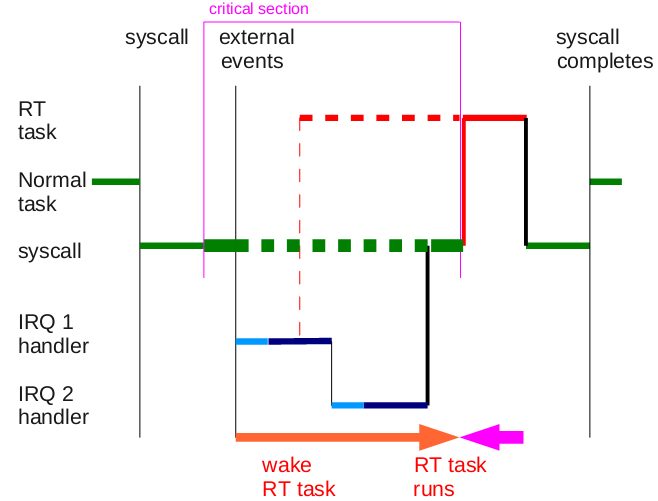
\includegraphics[width=12cm]{./figure/linux_rt_4type_preempt.png}
%  \caption{Linux的4类抢占区间}\label{linux_rt_4type_preempt}
%\end{figure}

\section{Linux实时补丁的用法}
linux的RT版本,https://wiki.linuxfoundation.org/realtime/start 这个项目是实现Linux的实时版本。主要原理是将Linux的中断线程化,即把一二三类区间都转换成四类区间。相应的linux 源码RT版本只针对特定的几个版本,使用方法是将代码中的RT补丁merge到对应的源码中,linux的RT可以做到100us量级的实时性能,(vxworks是几个us),相应的吞吐性能也会下降。

安装linux的调度器的抢占模型选项
\begin{enumerate}
  \item server版本 (不抢占)
  \item desktop版本 (kernel 内不抢占)
  \item no-latency desktop (kernel 内可抢占,手机桌面一般用此模型)
  \item completely preemption (kernel 内一二三类中断软中断都可抢占)
\end{enumerate}


安装RT补丁后还是会有很多的代码坑需要处理,比如内存管理方面,Linux的内存分配是LAZY式,当用到时才实际分配,安装实时补丁后有可能出现写内存时内存实际还未分配的情形。

\begin{example*}
  \wdexpbox
  {\caption{单反上的实时系统应用}}
  {实时系统的另一个应用场景是安装2个系统:实时系统和Linux,比如单反之前用的都是实时操作系统,现在为了增加蓝牙,wifi等功能,用一个核执行实时系统,另一个核用Linux来实现蓝牙等功能}
\end{example*}

%%% Local Variables:
%%% TeX-master: "main"
%%% End:
